\chapter{अंगजनन: चतुष्पाद अंग का निर्माण}\label{ch:b2:limb-organogenesis}

मुर्ग़ी का अंडा दिए जाने के तीन दिन बाद उस भ्रूण के हर पार्श्व पर
आलपिन के सिरे जितना एक उभार दिखता है। चार दिन बाद वह एक पंख है, जिसमें
एक प्रगंडिका, एक अरत्निका तथा अंतःप्रकोष्ठिका, एक कलाई और तीन अंगुलियाँ
हैं, सही क्रम में, सही लंबाइयों की, और पेशियाँ सही अस्थियों से जुड़ी हुई।
उस उभार के मोटी त्वचा वाले किनारे को काट दीजिए और वह पंख बढ़ना बंद कर
देता है; उसके पिछले किनारे की एक फाँक उसके अगले किनारे पर ग्राफ़्ट कर
दीजिए और वह दर्पण-प्रतिबिंब में छह अंगुलियाँ उगा लेता है। \omterm{def:b2:limb-organogenesis:bud}{अंग-कलिका}
\emph{अंगजनन} का उत्कृष्ट उदाहरण है --- यानी कोशिकाओं के किसी क्षेत्र से
ऐसे संकेतों द्वारा किसी अंग का निर्माण जो बताते हैं कि हर कोशिका कितनी
बाहर, कितनी आगे और कितनी ऊपर है --- और जिन प्रयोगों ने उसे खोला वे
जीवविज्ञान के सबसे स्पष्ट प्रयोगों में हैं। यह अध्याय उस कलिका का उसके
उभार से उसके कंकाल तक पीछा करता है।

\section{कलिका और उसकी तीन अक्षें}

\begin{definition}[अंग-कलिका]\label{def:b2:limb-organogenesis:bud}
\index{अंग-कलिका}\index{शीर्षस्थ बाह्यचर्मी कटक}\index{ध्रुवणकारी सक्रियता क्षेत्र}
\emph{अंग-कलिका} बाह्यचर्म से ढके \emph{पार्श्व पट्ट मध्यचर्म} की एक
सूजन है, जो पार्श्व पर किसी नियत स्थिति पर उठती है
(यानी \emph{अंग-क्षेत्र} पर) जहाँ शरीर-अक्ष का Hox कूट उसकी अनुमति देता
है; उसका मध्यचर्म अस्थि, उपास्थि, कंडरा और चर्म बनाएगा, और जो
कोशिकाएँ कायखंडों से उसमें प्रवास करती हैं वे पेशियाँ बनाएँगी।
उस कलिका की तीन अक्षें हैं, और हर एक को कोई संकेतन-केंद्र चलाता है।
\emph{समीपस्थ-दूरस्थ} (कंधे से अंगुली की नोक तक): \emph{शीर्षस्थ
बाह्यचर्मी कटक} (AER), यानी सिरे के साथ बाह्यचर्म की एक मोटी पट्टी,
\omterm{prop:b2:limb-organogenesis:aer}{तंतुकोरक वृद्धि कारक} (FGF) स्रावित करती है जो अपने नीचे के
मध्यचर्म को विभाजित होता और अविभेदित बनाए रखते हैं।
\emph{अग्र-पश्च} (अँगूठे से कनिष्ठिका तक): \emph{ध्रुवणकारी
सक्रियता क्षेत्र} (ZPA), यानी पिछले किनारे पर मध्यचर्म का एक खंड,
आकारजन \emph{\omterm{prop:b2:limb-organogenesis:zpa}{Sonic hedgehog}} (Shh) स्रावित करता है।
\emph{पृष्ठ-अधर} (हथेली की पीठ से हथेली तक): पृष्ठीय
बाह्यचर्म Wnt7a स्रावित करता है। अग्र-अंग और पश्च-अंग की कलिकाएँ एक जैसी
दिखती हैं और वही संकेत काम में लेती हैं; वे उस अनुलेखन कारक में भिन्न हैं
जो कलिका के प्रकट होने से पहले अभिव्यक्त होता है (अग्र-अंग में Tbx5,
पश्च-अंग में Tbx4), और इसीलिए पंख पंख है।
\end{definition}

\begin{omfigure}
\begin{tikzpicture}[every node/.style={font=\scriptsize}, >=stealth]
  % flank
  \fill[omExo!25] (0,-2.2) rectangle (1.2,2.2); \node[rotate=90] at (0.6,0) {देह-भित्ति (पार्श्व)};
  % bud outline: paddle
  \draw[thick, fill=omDef!10] (1.2,1.4) .. controls (3.0,1.9) and (5.2,1.6) .. (5.8,0.3) .. controls (5.9,-0.3) and (5.2,-1.6) .. (3.4,-1.7) .. controls (2.4,-1.8) and (1.6,-1.5) .. (1.2,-1.4);
  % AER along the tip
  \draw[line width=3pt, omThm] (5.2,1.3) .. controls (5.9,0.6) and (5.9,-0.6) .. (5.0,-1.4);
  \node[omThm, anchor=west, align=left] at (6.1,0.9) {शीर्षस्थ बाह्यचर्मी कटक (AER):\\FGF, समीपस्थ-दूरस्थ उभार};
  % ZPA posterior
  \draw[thick, omProp, fill=omProp!50] (2.4,-1.1) ellipse (0.55 and 0.4);
  \draw[omProp] (2.4,-1.5) -- (2.4,-2.0);
  \node[omProp, anchor=north, align=center] at (2.6,-2.0) {ZPA (पिछला किनारा):\\Sonic hedgehog, अग्र-पश्च};
  % dorsal ectoderm
  \draw[line width=2pt, omDef!70!black] (1.4,1.55) .. controls (3.0,2.0) and (5.0,1.7) .. (5.4,1.2);
  \node[omDef!70!black, anchor=south] at (3.4,2.05) {पृष्ठीय बाह्यचर्म: Wnt7a, पृष्ठ-अधर};
  % axes
  \draw[->, thick] (1.5,-3.1) -- (5.5,-3.1); \node[below] at (3.5,-3.15) {समीपस्थ $\to$ दूरस्थ};
  \draw[->, thick] (10.6,-1.6) -- (10.6,1.2); \node[right, align=left] at (10.7,-0.2) {पश्च $\to$ अग्र\\(कनिष्ठिका से अँगूठे तक)};
\end{tikzpicture}

{\small ऊपर से चूज़े की \omterm{def:b2:limb-organogenesis:bud}{अंग-कलिका}, अपने तीनों संकेतन-केंद्रों
सहित: सिरे के साथ का AER उभार चलाता है, पिछले किनारे का ZPA
अंगुलियों को ढाँचा देता है, और पृष्ठीय बाह्यचर्म पीठ को
हथेली से अलग करता है।}
\end{omfigure}

\begin{omfigure}
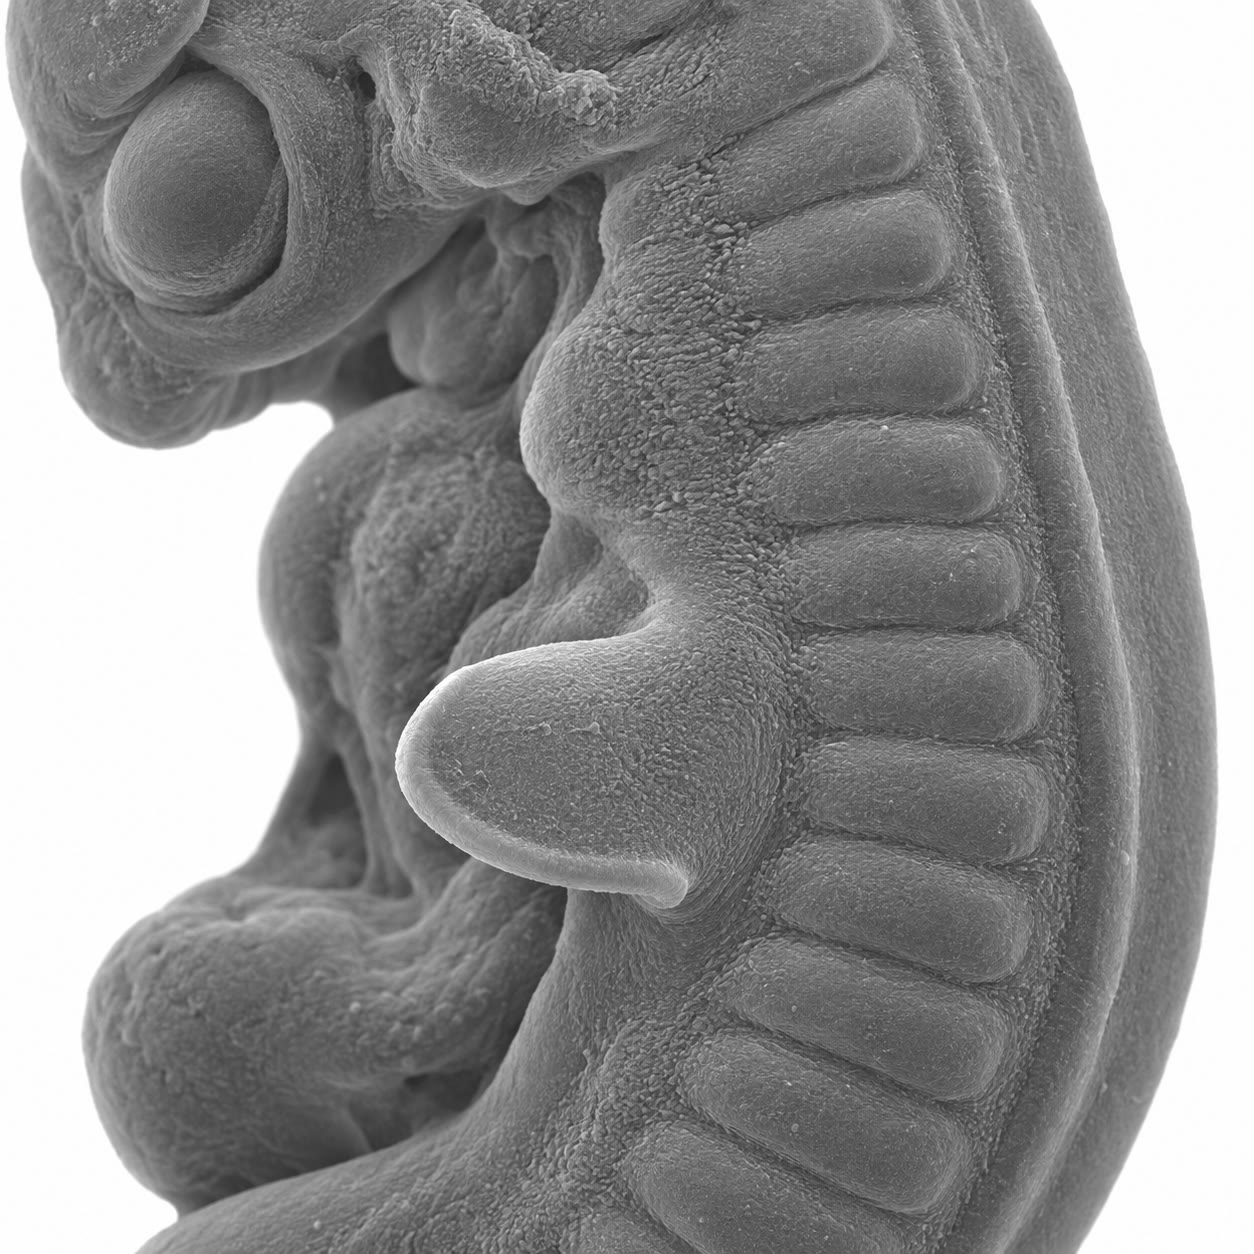
\includegraphics[width=0.42\linewidth]{images/book4/ai/b4-11-limb-bud.jpg}

{\small क्रमवीक्षी इलेक्ट्रॉन सूक्ष्मदर्शी के नीचे कोई चूज़ा-भ्रूण: धड़
के साथ कायखंडों की पंक्ति और, पार्श्व पर, चप्पू के आकार की
\omterm{def:b2:limb-organogenesis:bud}{अंग-कलिका}, जिसके किनारे के साथ मोटा कटक है।}
\end{omfigure}

\section{उभार: समीपस्थ-दूरस्थ अक्ष}

\begin{proposition}[शीर्षस्थ बाह्यचर्मी कटक]\label{prop:b2:limb-organogenesis:aer}
\index{तंतुकोरक वृद्धि कारक}\index{प्रगति क्षेत्र}
उभार के लिए AER आवश्यक है और उसके FGF पर्याप्त: उसके नीचे का
मध्यचर्म, यानी \emph{\omterm{prop:b2:limb-organogenesis:aer}{प्रगति क्षेत्र}}, कोई बारह
घंटे पर विभाजित होता है, और जो कोशिकाएँ सिरे के आगे बढ़ने पर उस क्षेत्र
से निकल जाती हैं वे विभाजित होना बंद कर देती हैं, संघनित होती हैं और
विभेदित हो जाती हैं। कंकाल समीपस्थ-दूरस्थ क्रम में बनता है ---
\emph{स्टाइलोपोड} (प्रगंडिका या ऊर्विका),
\emph{ज़्यूगोपोड} (अरत्निका और अंतःप्रकोष्ठिका, अंतर्जंघिका और
बहिर्जंघिका), \emph{ऑटोपोड} (कलाई और अंगुलियाँ) --- और हर खंड कलिका के
बढ़ने के साथ बारी-बारी निर्दिष्ट होता है, तथा वे खंड Hox जीन-अभिव्यक्ति
के नेस्टेड प्रांतों के संगत हैं (स्टाइलोपोड में Hoxa/d 9--10,
ज़्यूगोपोड में 11, ऑटोपोड में 13)। कोई \omterm{def:b2:limb-organogenesis:bud}{अंग-कलिका} चार दिनों में
लंबाई में कोई दस गुना बढ़ती है जबकि उस कटक के संकेत की पहुँच वही कुछ सौ
माइक्रोमीटर बनी रहती है, इसलिए वह कटक उस अंग को एक साथ नहीं बल्कि किसी
चलते मोर्चे की तरह ढाँचा देता है, जैसे कोई मुद्रक किसी पृष्ठ को
पंक्ति-दर-पंक्ति उतारता है।
\end{proposition}
\begin{proof}[प्रमाण-सामग्री]
सॉन्डर्स (1948) ने चूज़े की पंख-कलिकाओं से क्रमिक अवस्थाओं पर AER हटाया:
जल्दी हटाने पर उस कलिका ने केवल प्रगंडिका का ठूँठ दिया;
एक दिन बाद हटाने पर प्रगंडिका और प्रकोष्ठ, पर कोई हाथ नहीं; और उससे भी
बाद हटाने पर लगभग पूरा पंख --- यानी संक्रिया जितनी देर से, विच्छेद का
स्तर उतना ही दूरस्थ, इसलिए हर खंड के लिए बारी-बारी वह कटक चाहिए। दूसरा
कटक ग्राफ़्ट करने पर दूसरा उभार बना; और जिस कलिका का कटक हटाया गया था
उस पर FGF में भिगोया एक मनका रखने पर पूरा अंग बहाल हो गया (निसवैंडर,
1993), तथा अंग-क्षेत्रों के बीच पार्श्व पर रखे मनके ने एक अतिरिक्त अंग
प्रेरित कर दिया। जिन चूहों में कटक के FGF नहीं होते उनके अंग ही नहीं होते।
\end{proof}

\begin{omfigure}
\begin{tikzpicture}[every node/.style={font=\scriptsize}]
  \foreach \x/\lab/\n in {0/{AER जल्दी हटाया:\\केवल प्रगंडिका}/1, 3.6/{एक दिन बाद हटाया:\\प्रगंडिका, अरत्निका, अंतःप्रकोष्ठिका}/2, 7.2/{और बाद में हटाया:\\लगभग पूरा पंख}/3, 10.8/{अक्षत:\\पूरा पंख}/4} {
    \begin{scope}[xshift=\x cm]
      \fill[omExo!25] (0,-0.5) rectangle (0.5,2.6);
      % humerus
      \draw[thick, fill=omDef!25, rounded corners=3pt] (0.6,0.9) rectangle (1.7,1.2);
      \ifnum\n>1 \draw[thick, fill=omDef!25, rounded corners=3pt] (1.8,1.05) rectangle (2.7,1.3); \draw[thick, fill=omDef!25, rounded corners=3pt] (1.8,0.75) rectangle (2.7,1.0); \fi
      \ifnum\n>2 \foreach \y in {0.55,0.85,1.15} \draw[thick, fill=omDef!25, rounded corners=2pt] (2.8,\y) rectangle (3.3,\y+0.2); \fi
      \ifnum\n=4 \foreach \y in {0.55,0.85,1.15} \draw[thick, fill=omDef!25, rounded corners=2pt] (3.35,\y) rectangle (3.5,\y+0.2); \fi
      \node[below, align=center] at (1.8,-0.2) {\lab};
    \end{scope}
  }
\end{tikzpicture}

{\small सॉन्डर्स का प्रयोग। वह कटक जितनी जल्दी हटाया जाए, उस अंग का
उतना ही अधिक भाग नदारद रहता है, और वह भी सदा सिरे से: यानी हर खंड के
बिछते समय उसके लिए वह कटक चाहिए।}
\end{omfigure}

\begin{theorem}[विभाजन से वृद्धि]\label{thm:b2:limb-organogenesis:growth}
जिस कलिका की कोशिकाएँ हर $T$ घंटे पर विभाजित हों वह अपनी
कोशिका-संख्या $2^{t/T}$ गुना कर लेती है, किसी काल $t$ में; और बारह-घंटे चक्रों के चार दिन
$2^{8} = 256$ देते हैं। यदि उन चार दिनों में उस कलिका का आयतन हज़ार गुना
बढ़े, तो विभाजन 256 का गुणक जुटाता है और बाक़ी
चार का गुणक कोशिकाओं के बड़े होने से और उस आधात्री से आना चाहिए जो
उपास्थि कोशिकाएँ अपने चारों ओर स्रावित करती हैं। इसके विपरीत, जिस
खंड को निर्दिष्ट होने में एक कोशिका-चक्र लगे --- यानी वही मोटे तौर पर
बारह घंटे जिनसे सॉन्डर्स के प्रयोग के क्रमिक विच्छेद-स्तर अलग हैं ---
वह \omterm{prop:b2:limb-organogenesis:aer}{प्रगति क्षेत्र} के एक दुगुनेपन के संगत है।
\end{theorem}
\begin{proof}
$N(t) = N_0 2^{t/T}$; और $t = \qty{96}{h}$ तथा $T = \qty{12}{h}$ के साथ
$t/T = 8$। आवश्यक गुणक का विभाजन-गुणक से अनुपात,
$1000/256 \approx 4$, वही है जो विभाजन से भिन्न वृद्धि को
जुटाना पड़ता है।
\end{proof}

\section{अंगुलियाँ: अग्र-पश्च अक्ष}

\begin{proposition}[ध्रुवणकारी सक्रियता क्षेत्र]\label{prop:b2:limb-organogenesis:zpa}
\index{Sonic hedgehog}\index{आकारजन!Shh}
ZPA निर्दिष्ट करता है कि कौन-सी अंगुली कहाँ बनेगी। उसकी कोशिकाएँ
\omterm{prop:b2:limb-organogenesis:zpa}{Sonic hedgehog} स्रावित करती हैं, जो पिछले किनारे से उस कलिका के
आरपार फैलता है, और मध्यचर्म की कोशिकाएँ उसकी सांद्रता को --- और जितनी
देर वे उसके सामने रही हैं उसे भी --- किसी स्थिति के रूप में पढ़ती हैं:
सबसे ऊँची मात्रा सबसे पश्च अंगुली देती है, नीची मात्राएँ अधिक अग्र, और
किसी देहली से नीचे कोई अंगुली नहीं। उस प्रवणता का रूप
\cref{ch:b2:vertebrate-development} वाला चरघातांकी है, जिसकी क्षय-लंबाई
कुछ दहाई माइक्रोमीटर है, और उसकी देहलियाँ उस कलिका को
अंगुलियों के प्राथमिकांगों में काट देती हैं: चूज़े के पंख में, पश्च से
अग्र तक, अंगुलियाँ 4, 3 और 2। अगले किनारे पर उसी संकेत का दूसरा स्रोत
एक दूसरा, दर्पण-प्रतिबिंबी समुच्चय बना देता है; और कोई कमज़ोर स्रोत, या
कोई छोटा अनावरण, उस अतिरिक्त समुच्चय की केवल अग्र अंगुलियाँ बनाता है।
वही जीन, वही भूमिका निभाते हुए, हर चतुष्पाद की अंगुलियों को ढाँचा देता
है, और जो \omterm{def:b2:genome-diversification:mutation}{उत्परिवर्तन} Shh का कोई अग्र स्रोत जोड़ देता है वह
बिल्लियों, मुर्ग़ियों, चूहों और मनुष्यों में बहुअंगुलिता देता है।
\end{proposition}
\begin{proof}[प्रमाण-सामग्री]
सॉन्डर्स और गैसलिंग (1968) ने चूज़े की एक पंख-कलिका के पिछले किनारे का
मध्यचर्म-खंड काटकर दूसरी कलिका के अगले किनारे पर ग्राफ़्ट किया:
उस पोषी ने 4-3-2-2-3-4 क्रम में छह अंगुलियों वाला पंख उगाया, यानी
बीच के इर्द-गिर्द दर्पण-प्रतिबिंब। टिकल (1975) ने दिखाया कि अतिरिक्त
अंगुलियों की संख्या ग्राफ़्ट की गई कोशिकाओं की संख्या पर निर्भर थी ---
यानी एक मात्रा। रिड्ल और टैबिन (1993) ने पाया कि वह ग्राफ़्ट किया ऊतक
जीन \emph{\omterm{prop:b2:limb-organogenesis:zpa}{Sonic hedgehog}} अभिव्यक्त करता था, कि वह जीन उस कलिका में और
कहीं अभिव्यक्त नहीं होता था, और कि उसे अभिव्यक्त करने को बनाई गई
कोशिकाएँ अग्र भाग पर ग्राफ़्ट किए जाने पर वही दर्पण-द्विगुणन फिर से बना
देती थीं; और उस प्रोटीन के मनके ने भी वही किया। जिन चूज़ा-उत्परिवर्तियों
में Shh का कोई अग्र अस्थानिक धब्बा होता है उनमें अतिरिक्त अग्र अंगुलियाँ होती हैं।
\end{proof}

\begin{omfigure}
\begin{tikzpicture}[every node/.style={font=\scriptsize}, >=stealth]
  % normal bud with gradient and digits
  \begin{scope}
    \fill[omExo!25] (0,-0.3) rectangle (0.4,3.3);
    \shade[bottom color=omProp!60, top color=white] (0.4,-0.3) rectangle (3.2,3.3);
    \draw[thick] (0.4,-0.3) rectangle (3.2,3.3);
    \draw[thick, omProp, fill=omProp!70] (0.9,0.1) ellipse (0.45 and 0.35); \node[omProp!80!black, anchor=west] at (1.4,0.1) {ZPA};
    \foreach \y/\d in {0.6/4, 1.5/3, 2.4/2} { \draw[thick, fill=omDef!25, rounded corners=2pt] (3.3,\y-0.12) rectangle (4.2,\y+0.12); \node[right] at (4.25,\y) {अंगुली \d}; }
    \node[below, align=center] at (2.0,-0.5) {सामान्य कलिका: पिछले किनारे से\\Shh, अंगुलियाँ 4-3-2};
    \draw[->, thick] (-0.4,0.2) -- (-0.4,3.0); \node[rotate=90] at (-0.7,1.6) {पश्च $\to$ अग्र};
  \end{scope}
  % grafted bud
  \begin{scope}[xshift=7cm]
    \fill[omExo!25] (0,-0.3) rectangle (0.4,3.3);
    \shade[bottom color=omProp!60, top color=white] (0.4,-0.3) rectangle (3.2,1.5);
    \shade[top color=omProp!60, bottom color=white] (0.4,1.5) rectangle (3.2,3.3);
    \draw[thick] (0.4,-0.3) rectangle (3.2,3.3);
    \draw[thick, omProp, fill=omProp!70] (0.9,0.1) ellipse (0.45 and 0.35);
    \draw[thick, omProp, fill=omProp!70] (0.9,2.9) ellipse (0.45 and 0.35); \node[omProp!80!black, anchor=west] at (1.4,2.9) {ग्राफ़्ट किया ZPA};
    \foreach \y/\d in {0.3/4, 0.8/3, 1.3/2, 1.7/2, 2.2/3, 2.7/4} { \draw[thick, fill=omDef!25, rounded corners=2pt] (3.3,\y-0.1) rectangle (4.2,\y+0.1); \node[right] at (4.25,\y) {\d}; }
    \node[below, align=center] at (2.0,-0.5) {ZPA अग्र भाग पर ग्राफ़्ट किया:\\दर्पण-द्विगुणन 4-3-2-2-3-4};
  \end{scope}
\end{tikzpicture}

{\small ध्रुवणकारी क्षेत्र। बाएँ: Shh पिछले किनारे से फैलता है और
उसकी गिरती सांद्रता अंगुलियाँ 4, 3 और 2 निर्दिष्ट करती है।
दाएँ: अगले किनारे पर ग्राफ़्ट किया दूसरा ZPA एक दूसरी
प्रवणता और अंगुलियों का दर्पण-प्रतिबिंबी समुच्चय बना देता है।}
\end{omfigure}

\begin{theorem}[प्रवणता से अंगुली-सीमाएँ]\label{thm:b2:limb-organogenesis:thresholds}
पिछले किनारे पर $c_0$ सांद्रता की Shh और $\lambda$ क्षय-लंबाई के साथ,
जिस अंगुली की देहली $T_i$ हो उसके क्षेत्र की सीमा उस किनारे से
$x_i = \lambda\ln(c_0/T_i)$ पर पड़ती है। $\lambda = \qty{50}{\micro m}$
और अंगुलियों 4, 3 तथा 2 के लिए $0.6$,
$0.25$ तथा $0.08$ गुना $c_0$ की देहलियों के साथ, वे क्षेत्र
$0$--$26$, $26$--$69$ और $69$--$126$ माइक्रोमीटर हैं, और
\qty{126}{\micro m} से आगे का ऊतक कोई अंगुली नहीं बनाता। स्रोत दुगुना
करने पर हर सीमा $\lambda\ln 2 = \qty{35}{\micro m}$ बाहर खिसक जाती है
--- और कुछ सौ माइक्रोमीटर की कलिका में यह अगले किनारे पर एक अंगुली
जोड़ने को पर्याप्त है; और अगले किनारे पर कोई दूसरा स्रोत वही क्षेत्र
उलटे क्रम में बिछा देता है।
\end{theorem}
\begin{proof}
$c(x) = c_0 e^{-x/\lambda}$ से, $c = T_i$ तब जब $x_i = \lambda
\ln(c_0/T_i)$: $50\ln(1/0.6) = 25.5$, $50\ln 4 = 69$, $50\ln 12.5 =
126$। $c_0$ की जगह $2c_0$ रखने पर $\lambda\ln 2$ हर $x_i$ में जुड़ जाता है।
\end{proof}

\begin{omfigure}
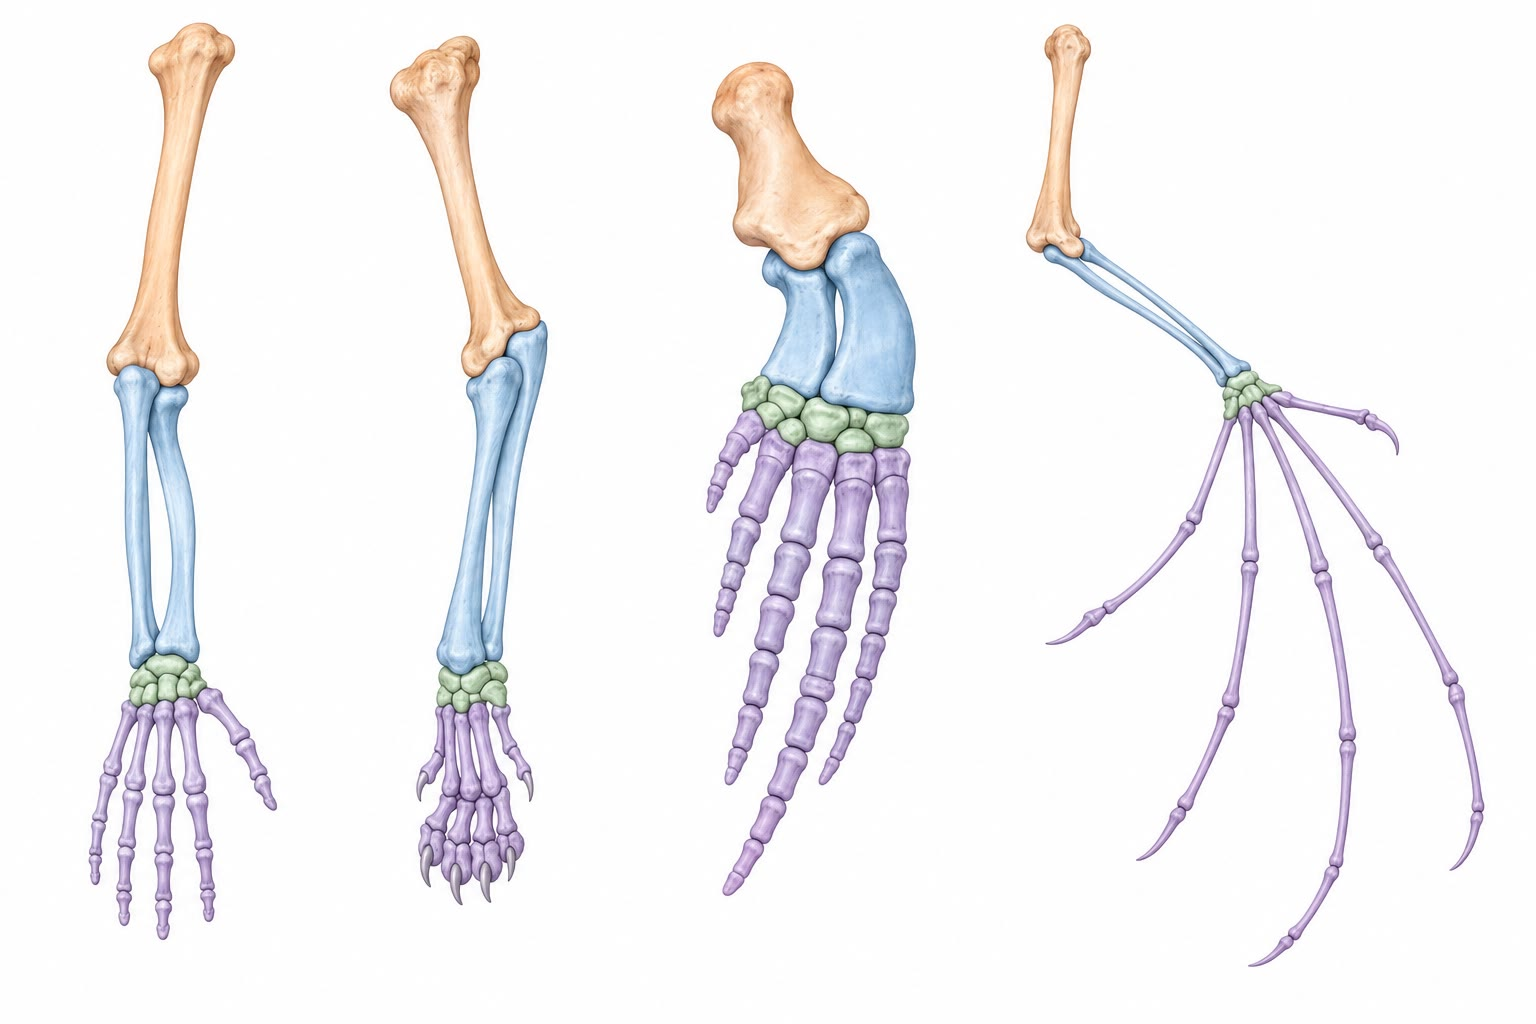
\includegraphics[width=0.66\linewidth]{images/book4/ai/b4-11-tetrapod-limbs.jpg}

{\small एक ही योजना, चार अंग: मनुष्य, बिल्ली, ह्वेल और चमगादड़ के
अग्र-अंगों में वही अस्थियाँ उसी क्रम में हैं --- एक
स्टाइलोपोड, दो ज़्यूगोपोड अस्थियाँ, कलाई, अंगुलियाँ --- जो उन्हीं
संकेतन-केंद्रों से गढ़ी गई हैं और केवल वृद्धि में भिन्न हैं।}
\end{omfigure}

\section{समन्वय और तराश}

\begin{proposition}[अक्षें आपस में बात करती हैं]\label{prop:b2:limb-organogenesis:loop}
\index{प्रतिपुष्टि चक्र!विकासात्मक}
वे केंद्र एक-दूसरे को बनाए रखते हैं: कटक की FGF ZPA को
Shh अभिव्यक्त करते रखती है, और Shh, मध्यचर्म के किसी रिले के रास्ते,
कटक को FGF अभिव्यक्त करते रखता है; किसी एक को हटा दीजिए और दूसरा दिन भर
में मिट जाता है। पृष्ठीय बाह्यचर्म की Wnt7a भी पूरी Shh
अभिव्यक्ति के लिए चाहिए, और वही मध्यचर्म की पृष्ठीय नियति चलाती है
(जिस चूहे में वह न हो उसकी दो हथेलियाँ होती हैं)। यह पारस्परिक निर्भरता
एक \emph{धन प्रतिपुष्टि चक्र} है जो तीनों अक्षों को आपस में बाँध देता है:
वह अंग वहीं बढ़ता है जहाँ उसे ढाँचा दिया जा रहा है, और उसे ढाँचा वहीं
दिया जाता है जहाँ वह बढ़ रहा है, इसलिए कोई कलिका कभी बिना बाँह के हाथ या
ग़लत क़िस्म की अंगुलियाँ नहीं बनाती। उभार पूरा हो जाने पर वह
चक्र टूट जाता है --- मध्यचर्म रिले करना बंद कर देता है, Shh रुक जाती है,
कटक क्षीण हो जाता है --- और वह अंग अपने उचित आकार पर बढ़ना बंद कर देता है।
\end{proposition}

\begin{proposition}[ढाँचे से अस्थि तक]\label{prop:b2:limb-organogenesis:skeleton}
\index{उपास्थिजनन}\index{कोशिका-मृत्यु!अंतरअंगुलीय}
एक बार निर्दिष्ट हो जाने पर \omterm{prop:b2:limb-organogenesis:aer}{प्रगति क्षेत्र} से निकलती मध्यचर्म कोशिकाएँ
भावी अस्थियों के आकार की छड़ों और पट्टिकाओं में \emph{संघनित} होती हैं,
उपास्थि कोशिकाओं में विभेदित होती हैं जो कोलैजन तथा प्रोटिओग्लाइकैन से
समृद्ध आधात्री स्रावित करती हैं, और हर कंकालीय अंश का उपास्थि-प्रतिरूप
बिछा देती हैं; संधियाँ वहाँ बनती हैं जहाँ कोशिकाओं की किसी पट्टी को
उपास्थि न बनने को कहा जाता है; रक्त वाहिकाएँ उन प्रतिरूपों पर आक्रमण
करती हैं और केंद्र से बाहर की ओर उपास्थि का स्थान अस्थि ले लेती है, और
सिरों पर वृद्धि-पट्टिकाएँ छूट जाती हैं जो उस अस्थि को वयस्कता तक लंबा
करती रहती हैं (\emph{उपास्थ्यंतर अस्थिभवन})। कायखंडों से
पेशी-पूर्वज भीतर प्रवास करते हैं, विभाजित होते हैं, तंतुओं में संलयित
होते हैं (\cref{ch:b2:cell-differentiation}) और उस अंग के अपने मध्यचर्म
की बनाई कंडराओं से जुड़ जाते हैं। अंगुली-किरणों के बीच का ऊतक
क्रमबद्ध कोशिका-मृत्यु से हटा दिया जाता है: अंतरअंगुलीय जालियों की
कोशिकाएँ, किसी अस्थि-आकारजनी प्रोटीन (BMP) के संकेत पर,
अपना ही विनाश चालू कर देती हैं और दिन भर में हटा दी जाती हैं, जिससे
अंगुलियाँ अलग हो जाती हैं। बत्तख़ अपनी जालियाँ इसलिए रखती है कि उसके
अंतरअंगुलीय ऊतक में कोई BMP संदमक अभिव्यक्त होता है; और किसी चूज़े को
मनके पर वही संदमक दिया जाए तो उसके जालीदार पैर उग आते हैं।
\end{proposition}
\begin{proof}[प्रमाण-सामग्री]
चूज़े की टाँग-कलिका से काटकर कहीं और ग्राफ़्ट किया गया अंतरअंगुलीय
मध्यचर्म समय पर ही मरता है --- यानी वह मृत्यु आंतरिक है, और ऊतक हटाए
जाने से पहले ही तय हो चुकी है; जबकि किसी बत्तख़ का वही ऊतक बचा रहता है।
बत्तख़ की अंगुलियों के बीच रखे BMP के मनके उस जाली को मार देते हैं;
और चूज़े की अंगुलियों के बीच रखे संदमक ग्रेम्लिन के मनके उसे बचा लेते
हैं। जिस चूहे में अंग का कोई BMP ग्राही न हो वह अपनी जालियाँ रखता है।
\end{proof}

\begin{omfigure}
\begin{tikzpicture}[every node/.style={font=\scriptsize}]
  \foreach \x/\lab in {0/{अंगुली-किरणें उपास्थि\\के रूप में संघनित}, 4.2/{अंतरअंगुलीय कोशिकाएँ\\मरती हैं (BMP)}, 8.4/{अंगुलियाँ अलग;\\उपास्थि की जगह अस्थि}} {
    \begin{scope}[xshift=\x cm]
      \node[below, align=center] at (1.5,-0.3) {\lab};
    \end{scope}
  }
  % stage 1: paddle with rays
  \draw[thick, fill=omDef!8] (0,0) .. controls (0,2.2) and (3,2.2) .. (3,0) -- cycle;
  \foreach \x in {0.6,1.2,1.8,2.4} \draw[thick, fill=omDef!30, rounded corners=2pt] (\x-0.12,0.1) rectangle (\x+0.12,1.5);
  % stage 2: paddle with dying webs
  \begin{scope}[xshift=4.2cm]
    \draw[thick, fill=omDef!8] (0,0) .. controls (0,2.2) and (3,2.2) .. (3,0) -- cycle;
    \foreach \x in {0.6,1.2,1.8,2.4} \draw[thick, fill=omDef!30, rounded corners=2pt] (\x-0.12,0.1) rectangle (\x+0.12,1.5);
    \foreach \x in {0.9,1.5,2.1} \foreach \y in {0.7,1.0,1.3} \fill[omThm] (\x,\y) circle (0.05);
  \end{scope}
  % stage 3: separated digits
  \begin{scope}[xshift=8.4cm]
    \draw[thick, fill=omDef!8] (0,0) -- (0,0.5) -- (0.3,0.5) -- (0.35,1.7) -- (0.85,1.7) -- (0.9,0.5) -- (1.05,0.5) -- (1.1,1.85) -- (1.6,1.85) -- (1.65,0.5) -- (1.8,0.5) -- (1.85,1.7) -- (2.35,1.7) -- (2.4,0.5) -- (2.7,0.5) -- (2.7,0) -- cycle;
    \foreach \x in {0.6,1.35,2.1} \draw[thick, fill=omExo!60, rounded corners=2pt] (\x-0.1,0.1) rectangle (\x+0.1,1.4);
  \end{scope}
\end{tikzpicture}

{\small हाथ की तराश: चप्पू में उपास्थि-किरणें संघनित होती हैं,
उनके बीच की कोशिकाएँ मरती हैं (लाल), और मुक्त हुई अंगुलियाँ अस्थिभूत होती हैं।}
\end{omfigure}

\begin{example}[वही अंग, भिन्न ढंग से उगाया हुआ]\label{ex:b2:limb-organogenesis:evolution}
चमगादड़ का पंख ऐसा हाथ है जिसकी अंगुलियाँ 2 से 5 किसी चूहे की अपेक्षा
कई गुना लंबी उगीं --- किसी अंग-जीन का एक संवर्धक, चमगादड़ से चूहे में
प्रत्यारोपित, चूहे की अग्र-अंग अस्थियाँ लंबी कर देता है --- और
जिसका अंतरअंगुलीय ऊतक बचा रहा, क्योंकि उस जाली में वही BMP संदमक
अभिव्यक्त होता है जो बत्तख़ काम में लेती है। ह्वेल का फ़्लिपर अतिरिक्त
अंगुलास्थियों वाला और बिना किसी अंतरअंगुलीय मृत्यु का हाथ है। घोड़े की
टाँग एक ही अंगुली है और बाक़ी घटकर खपच्चियाँ रह गई हैं। साँप के अंग
इसलिए नहीं हैं कि उसका पार्श्व वे संकेत कभी अभिव्यक्त ही नहीं करता जो
कोई कलिका आरंभ करते हैं। और मछलियों के पख, जिनमें ऑटोपोड नहीं होता, उसी
AER तथा ZPA से गढ़े जाते हैं पर अपना Hox कार्यक्रम उस पश्च प्रावस्था से
पहले रोक देते हैं जो अंगुलियाँ बनाती है; और जीवाश्म \emph{Tiktaalik}
(37.5 करोड़ वर्ष पुराना) किसी पख में कलाई को उभरते दिखाता है। अंग-विकास
अधिकतर किसी संरक्षित कार्यक्रम का परिवर्तन भर है --- कि हर प्रावस्था
कितनी देर चले, हर संकेत कितनी दूर पहुँचे, कौन-सी कोशिकाएँ मरें।
\end{example}

\section{अभ्यास}

\begin{exercise}[$\star$]\label{exo:b2:limb-organogenesis:1}
\omterm{def:b2:limb-organogenesis:bud}{अंग-कलिका} की तीनों अक्षें बताइए और हर एक के लिए संकेतन-केंद्र,
उसकी स्थिति और उसका संकेत।
\end{exercise}

\begin{exercise}[$\star$]\label{exo:b2:limb-organogenesis:2}
अंग-कंकाल के तीनों खंड और किसी मानव बाँह तथा टाँग में हर एक की
अस्थियाँ बताइए। उन्हें कौन-से Hox जीन चिह्नित करते हैं?
\end{exercise}

\begin{exercise}[$\star$]\label{exo:b2:limb-organogenesis:3}
पार्श्व पट्ट मध्यचर्म के किसी टुकड़े से लेकर अस्थि, संधि तथा पेशी सहित
किसी अंगुली तक के पग क्रम से बताइए।
\end{exercise}

\begin{exercise}[$\star$]\label{exo:b2:limb-organogenesis:4}
यदि AER हटाया जाए तो वह अंग कैसा दिखता है: (क) कलिका के प्रकट होते ही,
(ख) प्रकोष्ठ निर्दिष्ट हो जाने के बाद, (ग) बिलकुल नहीं हटाया जाए पर
FGF के किसी मनके से बदल दिया जाए?
\end{exercise}

\begin{exercise}[$\star\star$]\label{exo:b2:limb-organogenesis:5}
$\lambda = \qty{40}{\micro m}$ और अंगुलियों 4, 3 तथा 2 के लिए
स्रोत-सांद्रता की $0.5$, $0.2$ और $0.05$ देहलियों के साथ,
तीनों सीमाएँ और हर अंगुली-क्षेत्र की चौड़ाई निकालिए।
\end{exercise}

\begin{exercise}[$\star\star$]\label{exo:b2:limb-organogenesis:6}
चूज़े के पंख के अंगुली-प्रतिरूप की भविष्यवाणी कीजिए जब (क) पूरा ZPA
अगले किनारे पर ग्राफ़्ट किया जाए, (ख) उतनी ही कोशिकाओं के चौथाई का
ग्राफ़्ट, (ग) अगले किनारे पर Shh का कोई मनका छोटे अनावरण के बाद हटा
दिया जाए। हर एक को मात्रा और काल से समझाइए।
\end{exercise}

\begin{exercise}[$\star\star$]\label{exo:b2:limb-organogenesis:7}
किसी चूज़े की \omterm{def:b2:limb-organogenesis:bud}{अंग-कलिका} में कटक बनते समय \num{5000} कोशिकाएँ हैं और उसकी
कोशिकाएँ हर \qty{12}{h} पर विभाजित होती हैं। चार दिन बाद कितनी कोशिकाएँ?
यदि उस अवस्था पर उस अंग में $4\times 10^{6}$ कोशिकाएँ हों, तो
कोशिका-चक्र या कोशिका-मृत्यु के बारे में क्या सच होना चाहिए?
\end{exercise}

\begin{exercise}[$\star\star$]\label{exo:b2:limb-organogenesis:8}
समझाइए कि चूज़े की अंगुलियाँ मुक्त और बत्तख़ के पैर जालीदार क्यों हैं,
और किसी चूज़ा-भ्रूण की अंगुलियों के बीच BMP संदमक का मनका क्या करता है।
अंतरअंगुलीय मृत्यु का आंतरिक समय (वह किसी ग्राफ़्ट में भी समय पर होती
है) आपको बताता है कि उन कोशिकाओं को कैसे निर्देश मिला था?
\end{exercise}

\begin{exercise}[$\star\star$]\label{exo:b2:limb-organogenesis:9}
किसी चूहे में Hoxa13 और Hoxd13 दोनों नहीं हैं; और किसी दूसरे में
Hoxa11 तथा Hoxd11 नहीं। हर एक के अग्र-अंग के कंकाल की भविष्यवाणी कीजिए
और बताइए कि वह परिणाम Hox प्रांतों तथा खंडों के संबंध के बारे में क्या दिखाता है।
\end{exercise}

\begin{exercise}[$\star\star\star$]\label{exo:b2:limb-organogenesis:10}
AER और ZPA के बीच की धन प्रतिपुष्टि समझाइए, वह उस अंग को दृढ़ क्यों
बनाती है, और ऐसी किसी कलिका का क्या होगा जिसमें Shh FGF को बनाए न रख
सके। इसकी तुलना \cref{ch:b2:mammal-reproduction} की प्रसव वाली धन
प्रतिपुष्टि से कीजिए: हर चक्र को क्या समाप्त करता है?
\end{exercise}

\begin{exercise}[$\star\star\star$]\label{exo:b2:limb-organogenesis:11}
किसी चमगादड़ की तीसरी अंगुली शरीर-आकार के सापेक्ष किसी चूहे की अंगुली से
आठ गुना लंबी है। यदि अंगुली की उपास्थि किसी वृद्धि-खिड़की में $r$ दर से
चरघातांकी रूप से लंबी हो, और चमगादड़ की खिड़की चूहे की खिड़की से चार
दिन लंबी हो, तो कौन-सा $r$ चाहिए? दो विकासात्मक परिवर्तन बताइए (एक
वृद्धि में, एक कोशिका-मृत्यु में) जो किसी हाथ से एक पंख बना देते हैं।
\end{exercise}

\begin{exercise}[$\star\star\star$]\label{exo:b2:limb-organogenesis:12}
\omterm{prop:b2:limb-organogenesis:zpa}{Sonic hedgehog} तल-पट्ट से \omterm{prop:b2:vertebrate-development:neurulation}{तंत्रिका नली} को
(\cref{ch:b2:vertebrate-development}) और ZPA से अंगुलियों को ढाँचा देता
है। इस पर विचार कीजिए कि विकास थोड़े-से संकेत अनेक कामों के लिए क्यों
दोहराता है, वही अणु भिन्न ऊतकों में भिन्न अर्थ कैसे रख सकता है, और
ऐसे किसी जीन के \omterm{def:b2:genome-diversification:mutation}{उत्परिवर्तन} के प्रभाव के लिए इसका क्या अर्थ है।
\end{exercise}

\section{समस्या: सप्ताह भर में बना एक पंख}

\begin{problem}[{सप्तांत समस्या --- चूज़े के पंख का कलिका से कंकाल तक
पीछा: विभाजन से उसकी वृद्धि, सॉन्डर्स के कटक-निष्कासनों का समय, Shh
प्रवणता की गणना तथा उसके द्विगुणनों की भविष्यवाणी, जालियों की तराश और
उस पंख की किसी चमगादड़ के पंख से तुलना, और अंत दुगुनेपनों की संख्या,
अंगुली-सीमाओं और दर्पण-द्विगुणन के लिए आवश्यक चौड़ाई पर}]
\label{pb:b2:limb-organogenesis:1}
चूज़े की पंख-कलिका उद्भवन के 3 दिन पर \num{2000} मध्यचर्म कोशिकाओं और
\qty{0.4}{mm} लंबाई के साथ प्रकट होती है; और 7 दिन तक वह पंख
\qty{4}{mm} लंबा है तथा उसका आयतन उस कलिका के आयतन का \num{1000} गुना।
\omterm{prop:b2:limb-organogenesis:aer}{प्रगति क्षेत्र} की कोशिकाएँ हर \qty{12}{h} पर विभाजित होती हैं।
कटक-निष्कासन: 3.0 दिन पर वह अंग एक ठूँठ है; 3.5 दिन पर केवल एक
प्रगंडिका; 4.0 दिन पर प्रगंडिका, अरत्निका तथा अंतःप्रकोष्ठिका; और 4.5
दिन पर ऐसा पंख जिसमें केवल अंगुलियों के सिरे नहीं। Shh: $D = \qty{1e-12}{m^2/s}$,
अर्ध-जीवन \qty{29}{min}; और अंगुलियों 4, 3, 2 के लिए $0.6$,
$0.25$, $0.08$ गुना $c_0$ की देहलियाँ। कलिका की चौड़ाई (पश्च
से अग्र) \qty{600}{\micro m}। अंतरअंगुलीय जालियाँ: \qty{300}{\micro m}$\times$\qty{300}{\micro m}$\times$\qty{200}{\micro m} के तीन क्षेत्र, और
\qty{1000}{\micro m^3} की कोशिकाएँ, जो \qty{24}{h} में हटा दी जाती हैं।

\medskip
\noindent\textbf{भाग I --- वृद्धि।}
\begin{enumerate}
  \item चार दिनों में कितने दुगुनेपन होते हैं? \num{2000} से वे कितनी
        कोशिकाएँ देते हैं?
  \item हज़ार गुनी आयतन-वृद्धि से तुलना कीजिए: कोशिकाओं के बड़े होने
        और आधात्री को कौन-सा गुणक जुटाना पड़ता है?
  \item लंबाई कितने गुना बढ़ी? यदि वह कलिका अचर त्रिज्या के किसी बेलन
        की तरह बढ़ती, तो आयतन-गुणक क्या होता, और वह अंतर उसके आकार के
        बारे में क्या कहता है?
  \item कटक की FGF मध्यचर्म में \qty{300}{\micro m} भीतर तक पहुँचती है।
        3 दिन पर और 7 दिन पर उस कलिका का कितना अंश उसके प्रभाव में है?
  \item समझाइए कि किसी बढ़ते अंग में नियत पहुँच का कोई संकेत
        समीपस्थ-दूरस्थ अनुक्रम क्यों बनाता है।
  \item कोई कोशिका 4 दिन पर \omterm{prop:b2:limb-organogenesis:aer}{प्रगति क्षेत्र} छोड़ती है। वह किस खंड में
        जाती है?
\end{enumerate}

\medskip
\noindent\textbf{भाग II --- खंडों का समय।}
\begin{enumerate}[resume]
  \item निष्कासन-शृंखला से वह काल दीजिए जिस तक हर खंड
        (स्टाइलोपोड, ज़्यूगोपोड, ऑटोपोड) निर्दिष्ट हो चुका होता है।
  \item क्रमिक खंडों के निर्देशन को कितने कोशिका-चक्र अलग
        करते हैं?
  \item उस परिणाम को \omterm{prop:b2:limb-organogenesis:aer}{प्रगति क्षेत्र} और
        Hox प्रांतों के पदों में समझाइए।
  \item जिस कलिका का कटक 3.5 दिन पर हटाया गया उस पर FGF का मनका
        रखा जाता है। उस अंग की भविष्यवाणी कीजिए।
  \item किसी अक्षत कलिका की पृष्ठीय सतह पर 3.5 दिन पर दूसरा कटक
        ग्राफ़्ट किया जाता है। भविष्यवाणी कीजिए।
  \item वह कलिका अनिश्चित काल तक बढ़ते रहने के बजाय 7 दिन पर बढ़ना क्यों
        बंद कर देती है?
\end{enumerate}

\medskip
\noindent\textbf{भाग III --- प्रवणता।}
\begin{enumerate}[resume]
  \item Shh के लिए $k$ और $\lambda$ निकालिए।
  \item तीनों अंगुली-सीमाएँ और क्षेत्र-चौड़ाइयाँ निकालिए।
  \item \qty{600}{\micro m} की किसी कलिका में वह अग्र क्षेत्र कितना
        चौड़ा है जो कोई अंगुली नहीं बनाता?
  \item कोई \omterm{def:b2:genome-diversification:mutation}{उत्परिवर्तन} Shh का निर्गत दुगुना कर देता है। सीमाएँ फिर से
        निकालिए और बताइए कि कोई अतिरिक्त अंगुली बनती है या नहीं और कौन-सी।
  \item अगले किनारे पर कोई ZPA ग्राफ़्ट किया जाता है। दोनों अंगुली-2
        क्षेत्रों के अतिव्यापन के बिना पूरा दर्पण-समुच्चय 4-3-2-2-3-4
        किस न्यूनतम कलिका-चौड़ाई पर संभव है? क्या चूज़े की कलिका इतनी
        चौड़ी है?
  \item यदि वह कलिका केवल \qty{200}{\micro m} चौड़ी होती तो उस
        प्रतिरूप की भविष्यवाणी कीजिए।
  \item ZPA के चौथाई का ग्राफ़्ट केवल 2-2-3-4 क्यों देता है?
\end{enumerate}

\medskip
\noindent\textbf{भाग IV --- तराश और विकास।}
\begin{enumerate}[resume]
  \item तीनों जालियों में कोशिकाओं की संख्या और सफ़ाई के दौरान
        कोशिका-मृत्यु की दर, कोशिकाएँ प्रति सेकंड में, निकालिए।
  \item बत्तख़ की अंतरअंगुलीय कोशिकाएँ कोई BMP संदमक अभिव्यक्त करती हैं।
        बत्तख़ की जाली में BMP के मनके के और चूज़े की जाली में उस
        संदमक के प्रभाव की भविष्यवाणी कीजिए।
  \item चमगादड़ की अंगुली-उपास्थि चार अतिरिक्त दिन \qty{0.5}{d^{-1}}
        की चरघातांकी दर से बढ़ती है। वह चूज़े की उपास्थि से कितने गुना
        लंबी है? पंख की झिल्ली बनाने वाला दूसरा परिवर्तन बताइए।
  \item किसी मछली की पख-कलिका में AER और ZPA हैं पर अंगुलियाँ नहीं।
        क्या नहीं है, और \emph{Tiktaalik} क्या दिखाता है?
  \item यदि वे जाली-कोशिकाएँ इसके बजाय \num{1000} संस्थापकों से
        \qty{12}{h} प्रति चक्र पर विभाजन से बनी होतीं, तो उन्हें बनाने
        में कितना समय लगता? उन्हें हटाने में लगते एक दिन से तुलना कीजिए।
  \item परिणाम बताइए: चार दिनों के दुगुनेपन, तीनों अंगुली-सीमाएँ,
        और दर्पण-द्विगुणन के लिए न्यूनतम चौड़ाई।
\end{enumerate}
\end{problem}
